\documentclass[10pt]{article}

\usepackage[utf8]{inputenc}
\usepackage{latexsym,amsfonts,amssymb,amsthm,amsmath}
\setlength{\parindent}{0in}
\setlength{\parskip}{\baselineskip}
\setlength{\oddsidemargin}{0in}
\setlength{\textwidth}{6.5in}
\setlength{\textheight}{8.8in}
\setlength{\topmargin}{0in}
\setlength{\headheight}{18pt}

\usepackage[a4paper,margin=1in,footskip=0.25in]{geometry}

\usepackage{listings}
\usepackage{color} %red, green, blue, yellow, cyan, magenta, black, white
\definecolor{mygreen}{RGB}{28,172,0} % color values Red, Green, Blue
\definecolor{mylilas}{RGB}{170,55,241}

\usepackage{graphicx}
\graphicspath{{../output/}}

\def\code#1{\texttt{#1}} % Monospacing shortcut: Use \code{}

\usepackage[colorlinks=true, urlcolor=blue, linkcolor=blue]{hyperref}

\usepackage{verbatim} % For including raw text files in the pdf
\usepackage{float} % For keeping figures in the section where they were called 

\title{PHYS 410 Homework 2}
\author{Gavin Pringle, 56401938}

%%%%%%%%%%%%%%%%%%%%%%%%%%%%%%%%%%%%%%%%%%%%%%%%%%%%%%%%%%%%%%%%%%%%%%%%%%%%%%%%%%%%%%%%%%%%%%%%%%%%%%%
% Start of document
%%%%%%%%%%%%%%%%%%%%%%%%%%%%%%%%%%%%%%%%%%%%%%%%%%%%%%%%%%%%%%%%%%%%%%%%%%%%%%%%%%%%%%%%%%%%%%%%%%%%%%%
\begin{document}

\maketitle

\lstset{language=Matlab,%
    %basicstyle=\color{red},
    breaklines=true,%
    morekeywords={matlab2tikz},
    keywordstyle=\color{blue},%
    morekeywords=[2]{1}, keywordstyle=[2]{\color{black}},
    identifierstyle=\color{black},%
    stringstyle=\color{mylilas},
    commentstyle=\color{mygreen},%
    showstringspaces=false,%without this there will be a symbol in the places where there is a space
    numbers=left,%
    numberstyle={\tiny \color{black}},% size of the numbers
    numbersep=9pt, % this defines how far the numbers are from the text
    emph=[1]{for,end,break},emphstyle=[1]\color{red}, %some words to emphasise
    %emph=[2]{word1,word2}, emphstyle=[2]{style},    
}

%%%%%%%%%%%%%%%%%%%%%%%%%%%%%%%%%%%%%%%%%%%%%%%%%%%%%%%%%%%%%%%%%%%%%%%%%%%%%%%%%%%%%%%%%%%%%%%%%%%%%%%
% Introduction
%%%%%%%%%%%%%%%%%%%%%%%%%%%%%%%%%%%%%%%%%%%%%%%%%%%%%%%%%%%%%%%%%%%%%%%%%%%%%%%%%%%%%%%%%%%%%%%%%%%%%%%
\subsection*{Introduction}

In this homework assignment, the fourth-order Runge-Kutta method for computing numerical solutions of 
ODEs is explored. This is done in stages, culminating in creating a MATLAB function that numerically
integrates an ODE using an algorithm that automatically varies the step size of the integrator in order
to achieve a relative error tolerance. 

First, a function \code{rk4step} is written that computes a single fourth-order Runge-Kutta step for a 
system of coupled first-order ODEs, returning the approximate values of the dependent variables after
a defined time step. The function \code{rk4step} is then used in the function \code{rk4} which computes 
the solution of an initial value problem over a range of values for the independent variable, done by 
taking multiple fourth-order Runge-Kutta steps in a loop. Lastly, the function \code{rk4ad} is written 
which finds the numerical solution of an initial value problem by comparing the results of fourth-order 
Runge-Kutta steps of different sizes and then varying the step size as until the error in the 
approximation is below a specified relative tolerance.

%%%%%%%%%%%%%%%%%%%%%%%%%%%%%%%%%%%%%%%%%%%%%%%%%%%%%%%%%%%%%%%%%%%%%%%%%%%%%%%%%%%%%%%%%%%%%%%%%%%%%%%
% Review of Theory
%%%%%%%%%%%%%%%%%%%%%%%%%%%%%%%%%%%%%%%%%%%%%%%%%%%%%%%%%%%%%%%%%%%%%%%%%%%%%%%%%%%%%%%%%%%%%%%%%%%%%%%
\subsection*{Review of Theory}

\subsubsection*{Casting systems of ODEs in first-order form}

In order to solve complicated ODEs numerically, it is useful to first cast them in a canonical form that 
is easier for a computer program to understand. Any ODE defining the function $y(t)$ that is of the form 
$$f(t, y, y', y'', y^{(3)}, \ldots,  y^{(N)}) = 0$$
can be rewritten as a system of $N$ coupled first-order ODEs for the functions 
$y_i(t), \quad i = 1, 2, 3, \ldots, N$:
\begin{equation}\label{sys_DE}
y_i'(t) \equiv \frac{dy_i}{dt}(t) = f_i(t, y_1, y_2, y_3, \ldots, y_N)
\end{equation}
where $f_i$ are known functions of $t$ and $y_i$. This is equivalent to
\begin{equation}\label{sys_DE_vec}
\mathbf{y'} = \mathbf{f}(t, \mathbf{y}) \quad \textrm{where} \quad \mathbf{y} \equiv (y_1, y_2, y_3, 
\ldots, y_N)
\end{equation}

For example, the function $y^{(4)}(t) = f(t)$ can be written as 
$$y_3' = f, \quad y' = y_1, \quad y_1' = y2, \quad y_2' = y_3$$

\subsubsection*{The fourth-order Runge-Kutta step}

The fourth-order Runge-Kutta step for numerically solving a system of $N$ coupled first-order ODEs is 
defined as:
\begin{equation}\label{rk_step}
y_i(t_0 + h) = y_i(t_0) + \frac{h}{6} (f_{0,i} + 2f_{1,i} + 2f_{2,i} + f_{3,i})
\end{equation}
with the terms $f_{0,i} \;f_{1,i} \;f_{2,i} \;f_{3,i}$ given by 
\begin{align}\label{rk_step_f_defs}
f_{0,i} &= f_i(t_0, \;y_{0,i}) \\
f_{1,i} &= f_i\left(t_0 + \frac{h}{2}, \;y_{0,i} + \frac{h}{2} f_{0,i}\right) \\
f_{2,i} &= f_i\left(t_0 + \frac{h}{2}, \;y_{0,i} + \frac{h}{2} f_{1,i}\right) \\
f_{3,i} &= f_i\left(t_0 + h, \;y_{0,i} + h f_{2,i}\right)
\end{align}
where each $f_i$ on the right-hand sides of the above equations are defined in (\ref{sys_DE}) and 
h is the step size. This can be understood as a weighted sum of four numerical approximations to the 
solution of the ODE. A single fourth-order Runge-Kutta step is accurate to $O(\Delta t^5)$.

%%%%%%%%%%%%%%%%%%%%%%%%%%%%%%%%%%%%%%%%%%%%%%%%%%%%%%%%%%%%%%%%%%%%%%%%%%%%%%%%%%%%%%%%%%%%%%%%%%%%%%%
% Numerical approach
%%%%%%%%%%%%%%%%%%%%%%%%%%%%%%%%%%%%%%%%%%%%%%%%%%%%%%%%%%%%%%%%%%%%%%%%%%%%%%%%%%%%%%%%%%%%%%%%%%%%%%%
\subsection*{Numerical Approach}

\subsubsection*{Consecutive fourth-order Runge-Kutta steps}

In order to compute the numerical solution to an ODE (or in canonical form, a system of first-order 
ODEs), multiple consecutive fourth-order Runge-Kutta steps must be taken. The MATLAB implementation of 
a single fourth-order Runge-Kutta step is shown in Appendix A as \code{rk4step.m}, while Appendix C 
shows the MATLAB implementation of a complete fourth-order Runge-Kutta ODE integrator as \code{rk4.m}. 
In \code{rk4.m}, equation (\ref{rk_step}) is repeatedly computed using the previous output of equation 
(\ref{rk_step}) as an input. The step size \code{dt} is given by the difference at the current time-step 
between independent variable values at which the solution of the ODE is to be computed at, passed as 
\code{tspan}.

It is important to note that while a single fourth-order Runge-Kutta step is accurate to $O(\Delta t^5)$,
the full numerical solution to and ODE given by \code{rk4.m} is accurate to $O(\Delta t^4)$, since
error accumulates linearly throughout the integration. 

\subsubsection*{Adaptive step sizing}

The Runge-Kutta integrator can be made more accurate by varying the step size \code{dt} at each step 
depending on an estimation of the error accumulated in that step. To show how the per-step error can be
estimated using time-steps of multiple lengths, consider (for each dependent variable y in the system of 
ODEs) a "coarse" step of length $\Delta t$ (producing the output $y_C$) and two "fine" steps of length 
$\Delta t / 2$ (producing the output $y_F$).
\begin{align*}\label{y_F_and_y_C}
y_C(t_0 + \Delta t) &\approx y_{\text{exact}}(t_0 + \Delta t) + k(t_0) \Delta t^5 \\
y_F(t_0 + \Delta t) &\approx y_{\text{exact}}(t_0 + \Delta t) + k(t_0) \left( \frac{\Delta t}{2} 
\right)^5 + k\left(t_0 + \frac{\Delta t}{2}\right) \left( \frac{\Delta t}{2} \right)^5 \\
&\approx y_{\text{exact}}(t_0 + \Delta t) + 2 k(t_0) \left( \frac{\Delta t}{2} \right)^5
\end{align*}
In the above equations, $k(t)$ is some function of time. Subtracting $y_F$ and $y_C$ at the advanced time,
we get
\begin{equation}\label{error_estimation}
y_C(t_0 + \Delta t) - y_F(t_0 + \Delta t) \approx \frac{15}{16}k(t_0) \Delta t^5 \approx \frac{15}{16}e_C
\end{equation}
which yields an estimate for the local solution error $e_C$.

This error estimation is implemented in the MATLAB function \code{rk4ad.m} (Appendix F), which functions 
as an adaptive step size fourth-order Runge-Kutta ODE integrator. In \code{rk4ad.m}, similar to 
\code{rk4.m}, the function is written to compute the values of the ODE defined by the argument \code{fcn}
at the times defined in \code{tspan}, with the initial values of the dependent variables defined by 
\code{y0}. However, the additional argument \code{reltol} is also passed which directs the function to 
iteratively decrease the step sizes in between values of \code{tspan} until the step-size to step-size 
error described above is below \code{reltol}. A lower bound for the step-size is defined by the constant 
\code{floor = 1.0e-4}.

At each time-step in \code{rk4ad.m}, the coarse numerical solution is computed using the distance to the 
next time-step and the fine numerical solution is computed using two time-steps equalling half the 
distance to the next time step. These solutions are then compared as shown in (\ref{error_estimation}). If 
the estimated solution error is above \code{reltol}, the process is repeated where each fine step is 
divided into two even finer steps and the solution across the four time steps is compared to the solution
across the two time steps. If the new estimated error is below \code{reltol}, the process stops and the 
function moves on to computing the solution at the next time-step, and if not the process of successively 
halving the step-size continues until either \code{reltol} is achieved or the step-size limit \code{floor}
is reached. 

%%%%%%%%%%%%%%%%%%%%%%%%%%%%%%%%%%%%%%%%%%%%%%%%%%%%%%%%%%%%%%%%%%%%%%%%%%%%%%%%%%%%%%%%%%%%%%%%%%%%%%%
% Implementation
%%%%%%%%%%%%%%%%%%%%%%%%%%%%%%%%%%%%%%%%%%%%%%%%%%%%%%%%%%%%%%%%%%%%%%%%%%%%%%%%%%%%%%%%%%%%%%%%%%%%%%%
\subsection*{Implementation}

\subsubsection*{ODE test functions} % sho and vdp

In order to test the functions \code{rk4step.m}, \code{rk4.m}, and \code{rk4ad.m}, sample ODEs must be
used. The first of the two ODEs used in this assignment to test the ODE integrators is the ODE for the
simple harmonic oscillator with unit angular frequency. This ODE is given by the following equation:
\begin{equation}\label{sho_ode}
\frac{d^2x}{dt^2}(t) = -x(t)
\end{equation}
with the initial conditions 
$$x(0) = 0, \quad \frac{dx}{dt}(0) = 1$$
In the canonical first-order form this ODE can be written as 
$$\frac{dx_1}{dt} = x_2, \quad \frac{dx_2}{dt} = -x_1$$
where 
$$x_1 = x, \quad x_2 = \frac{dx}{dt}$$
The function \code{fcn\_sho} was written to implement this ODE in MATLAB in order to pass it to 
\code{rk4.m} and \code{rk4ad.m}:
\begin{verbatim}
function dxdt = fcn_sho(t, x)
    dxdt = zeros(2,1);
    dxdt(1) = x(2);
    dxdt(2) = -x(1); 
end
\end{verbatim}

The second of the two ODEs used is the ODE for the unforced Van der Pol oscillator, shown below
\begin{equation}\label{vdp_ode}
\frac{d^2x}{dt^2}(t) = -x(t) - a(x(t)^2 - 1)\frac{dx}{dt}(t)
\end{equation}
In this assignment, $a = 5$ and the following initial conditions are used: 
$$x(0) = 1, \quad \frac{dx}{dt}(0) = -6$$
In the canonical first-order form this ODE can be written as 
$$\frac{dx_1}{dt} = x_2, \quad \frac{dx_2}{dt} = -x_1(t) - a(x_1(t)^2 - 1)x_2(t)$$
where 
$$x_1 = x, \quad x_2 = \frac{dx}{dt}$$
The function \code{vdp\_sho} was written to implement this ODE in MATLAB in order to pass it to 
\code{rk4.m} and \code{rk4ad.m}:
\begin{verbatim}
function dxdt = fcn_vdp(t, x)
    global a;
    dxdt = ones(2,1);
    dxdt(1) = x(2);
    dxdt(2) = -x(1) - a*(x(1)^2 - 1)*x(2);
end
\end{verbatim}

%%%%%%%%%%%%%%%%%%%%%%%%%%%%%%%%%%%%%%%%%%%%%%%%%%%%%%%%%%%%%%%%%%%%%%%%%%%%%%%%%%%%%%%%%%%%%%%%%%%%%%%
% Results
%%%%%%%%%%%%%%%%%%%%%%%%%%%%%%%%%%%%%%%%%%%%%%%%%%%%%%%%%%%%%%%%%%%%%%%%%%%%%%%%%%%%%%%%%%%%%%%%%%%%%%%
\subsection*{Results}

\subsubsection*{rk4step.m Output}

To test the functionality and accuracy of the single fourth-order Runge-Kutta step function
\code{rk4step.m}, the script \code{trk4step.m} was written, shown in Appendix B. The simple harmonic 
oscillator ODE is implemented as described previously, and the function \code{rk4step} is called 
repeatedly in a loop with an increasing step size defined by the array 
\code{dt = linspace(0.01, 0.3, 1000)} and the parameters \code{x0 = [0; 1]} and \code{t0 = 0}. The 
error between computed value of $y$ for each step size and the exact value given by 
$y(t + \Delta t) = \sin(t + \Delta t)$ was then plotted.  

By guessing and checking, the constant $C = 0.0083$ was found that causes the curve defined by 
$C \Delta t^5$ to align with the curve given by the error between the computed solutions and the 
exact solutions. Since this curve is proportional to $\Delta t^5$ as shown in Figure \ref{rk4step_fig},
we can conclude that a single step of the fourth-order Runge-Kutta integrator is accurate to 
$O(\Delta t^5)$.

\begin{figure}[H]
\centering
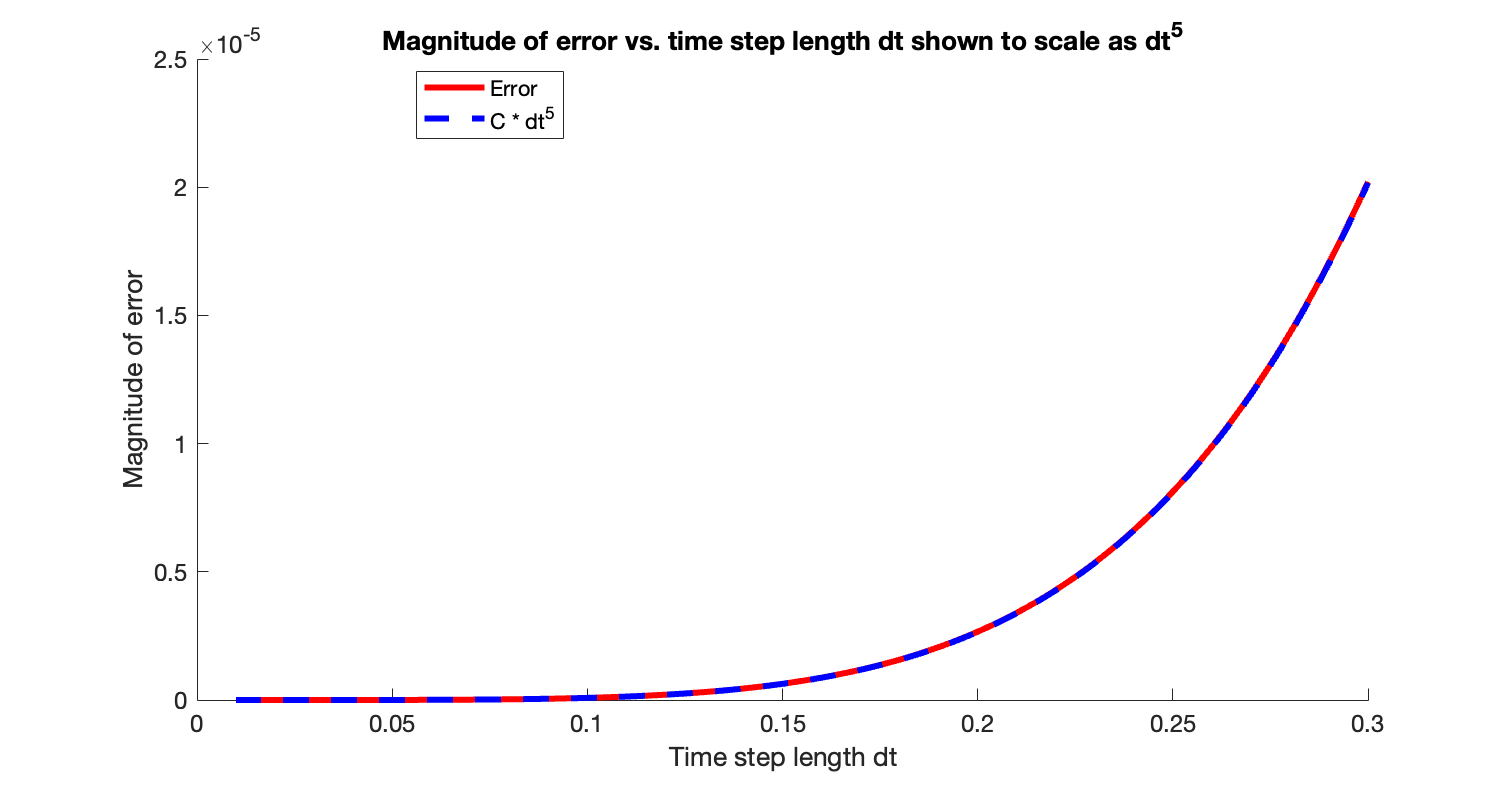
\includegraphics[width=0.9\textwidth]{rk4step.png}
\caption{Exact error of Runge-Kutta steps of various sizes for the simple harmonic oscillator ODE at 
\code{t0 = 0}. Alignment with the curve $0.0083 \times dt^5$ shows the error is proportional to 
$\Delta t^5$.}\label{rk4step_fig}
\end{figure}

\subsubsection*{rk4.m Output}

The function \code{rk4} was written to numerically integrate an ODE by taking consecutive 
Runge-Kutta steps, as described previously. To test this function, two scripts were written, the 
first being \code{trk4\_sho.m}, which calls \code{rk4} to integrate the simple harmonic oscillator 
ODE. This was done with the initial conditions defined by \code{x0 = [0; 1]} on the interval 
$0 \leq t \leq 3\pi$ at discretization levels $l = 6, 7, 8$. Since the exact solution to this IVP
is given by $y(t) = \sin(t)$, the exact errors were calculated for each discretization level.

For fourth order convergence, the magnitude of the error given by the numerical solutions is expected 
to decrease by a factor of $(2 \Delta l)^4$ for each increase $\Delta l$ above a baseline $l$. If we 
scale the errors at higher discretization levels by dividing by this value, we should see near 
convergence for the error curves if our approximation is accurate to $O(\Delta t^4)$. We can see in 
Figure \ref{trk4_sho_2_fig} that is the case as we expect. Refer to Appendix D for the MATLAB code 
for \code{trk4\_sho.m}.

\begin{figure}[H]
\centering
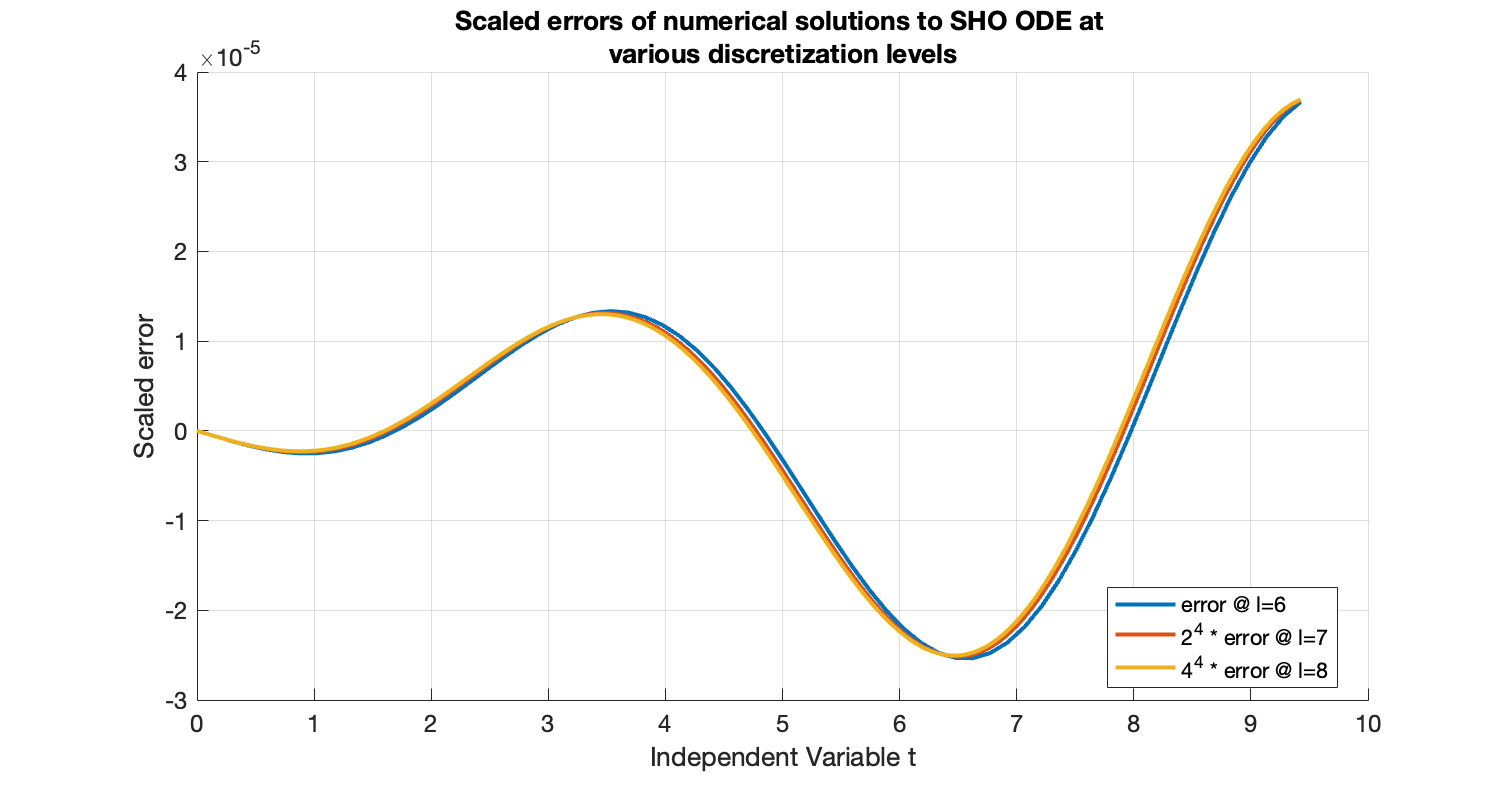
\includegraphics[width=0.9\textwidth]{trk4_sho_2.png}
\caption{Fourth-order convergence shown by near alignment of the exact errors of numerical solutions 
at different discretization levels, each scaled to show expected fourth-order convergence behaviour.
}\label{trk4_sho_2_fig}
\end{figure}

The second script written to test the function \code{rk4} is \code{trk4\_vdp.m}, which calls \code{rk4} 
to integrate the unforced Van der Pol oscillator ODE. This was done with the initial conditions defined 
by \code{x0 = [1; -6]} on the interval $0 \leq t \leq 100$ at discretization level 12. The numerical 
solution for the function $x(t)$ is plotted in Figure \ref{trk4_vdp_1_fig} and the phase space 
evolution $\frac{dx}{dt}(x)$ is plotted in Figure \ref{trk4_vdp_2_fig}. In view of the 
\href{https://en.wikipedia.org/wiki/Van_der_Pol_oscillator}{Wikipedia page} for the Van der Pol 
oscillator, we can confirm that this is the expected output which provides evidence that \code{rk4} has 
been implemented correctly. Refer to Appendix E for the MATLAB code for \code{trk4\_vdp.m}.

\begin{figure}[H]
\centering
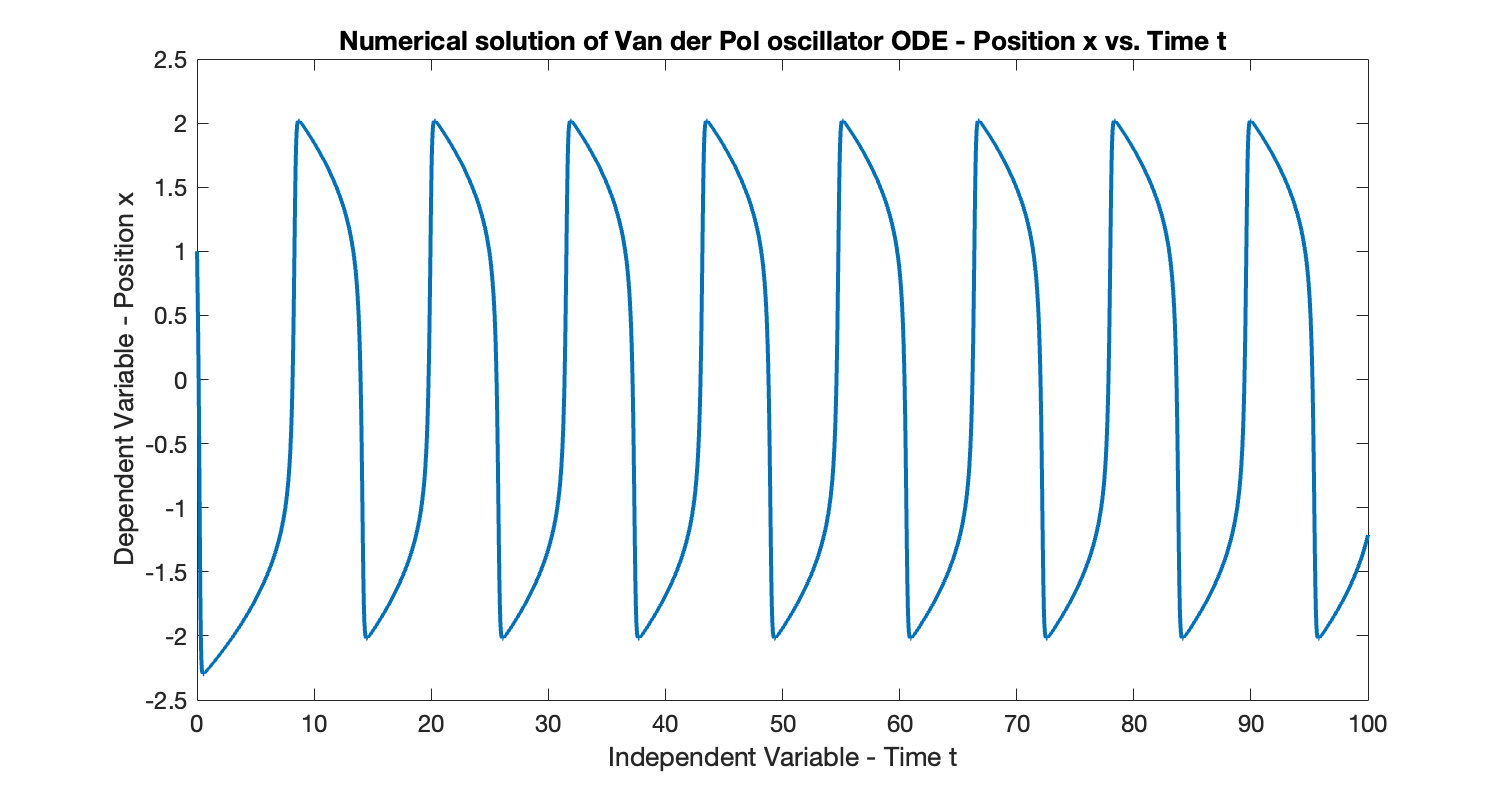
\includegraphics[width=0.9\textwidth]{trk4_vdp_1.png}
\caption{Numerical solution of the Van der Pol oscillator ODE computed by \code{rk4.m} on the domain
$0 \leq t \leq 100$ at discretization level 12.}\label{trk4_vdp_1_fig}
\end{figure}

\begin{figure}[H]
\centering
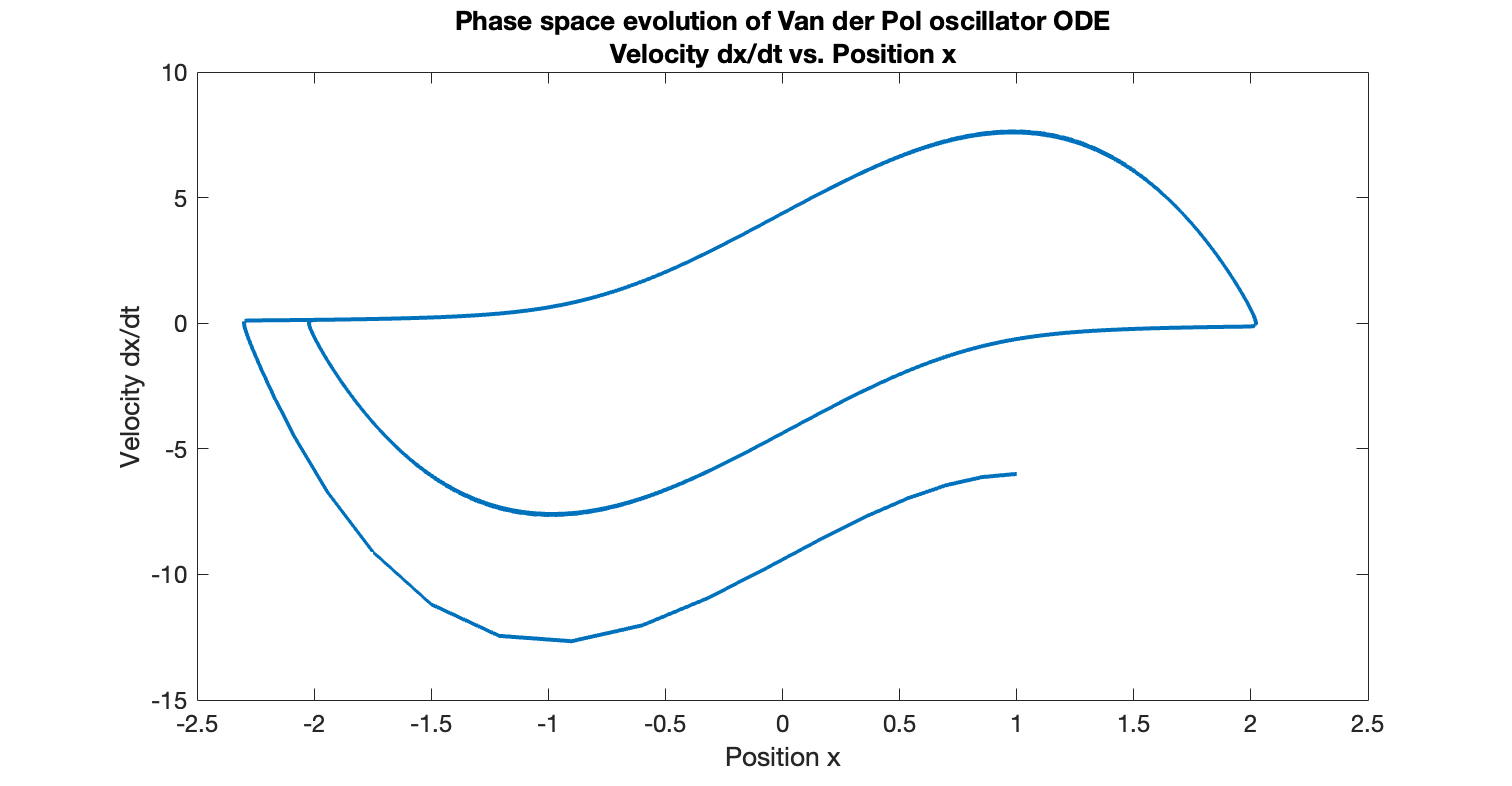
\includegraphics[width=0.9\textwidth]{trk4_vdp_2.png}
\caption{Phase space evolution of the Van der Pol oscillator ODE computed by \code{rk4.m} on the domain
$0 \leq t \leq 100$ at discretization level 12.}\label{trk4_vdp_2_fig}
\end{figure}

\subsubsection*{rk4ad.m Output}

The fourth-order Runge-Kutta ODE integrator described previously is implemented in the function 
\code{rk4ad}. To test this function, two scripts were again written, the first being \code{trk4\_sho.m}, 
which calls \code{rk4} to integrate the simple harmonic oscillator ODE. This script uses the function
parameter \code{x0 = [0; 1]} and \code{tspan = linspace(0.0, 3.0 * pi, 65)} to integrate the function 
four times with the relative tolerances \code{1.0e-5, 1.0e-7, 1.0e-9, 1.0e-11}. Figure 
\ref{trk4ad_sho_2_fig} shows the exact error of each approximation throughout the domain of $t$ upon 
which the ODE was integrated. It is clear that the numerical approximations rapidly become more 
accurate as \code{reltol} decreases, as expected. Refer to Appendix E for the MATLAB code for 
\code{trk4ad\_sho.m}.

\begin{figure}[H]
\centering
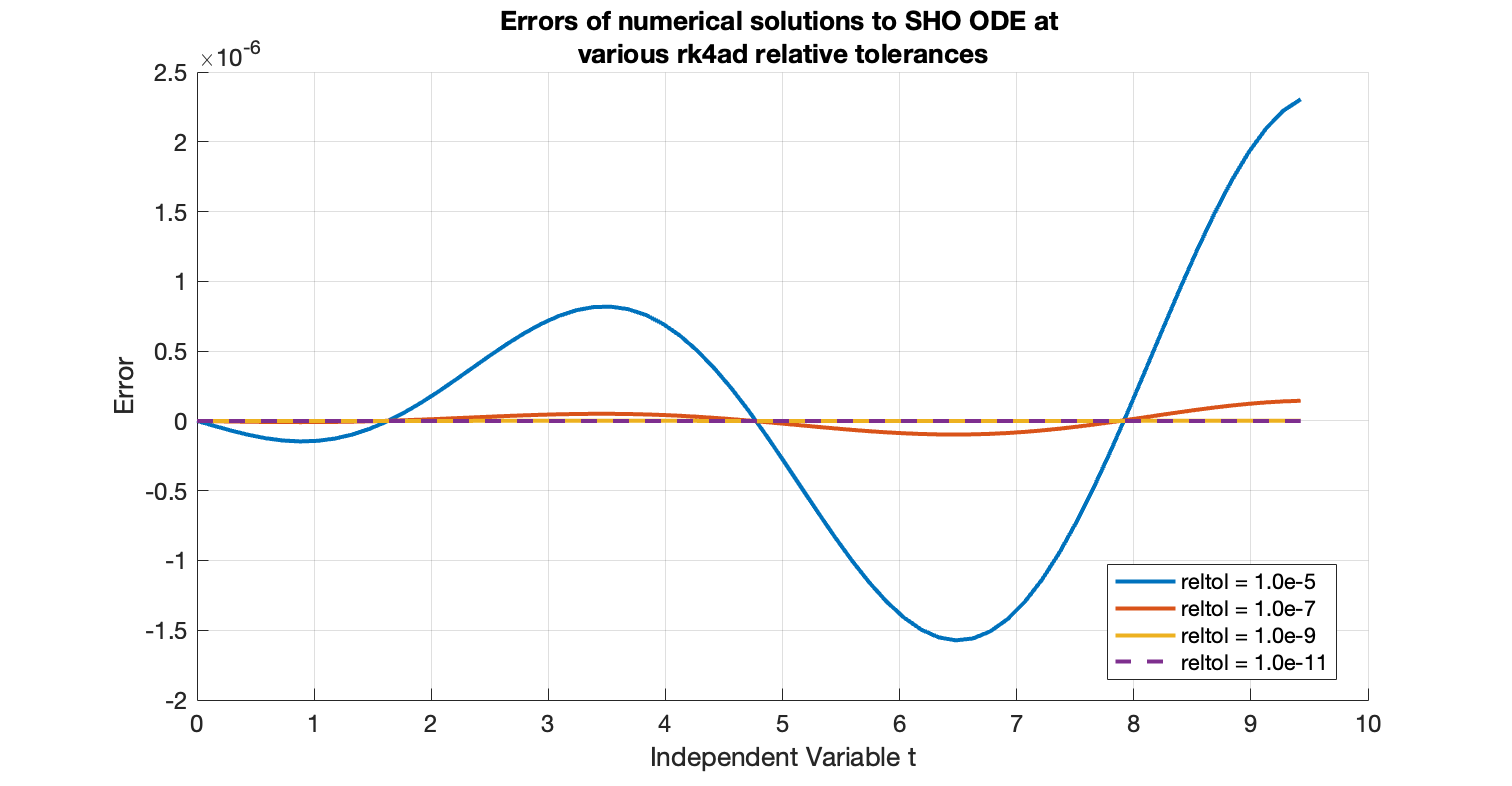
\includegraphics[width=0.9\textwidth]{trk4ad_sho_2.png}
\caption{Errors of numerical solutions to the simple harmonic oscillator ODE at various \code{rk4ad.m}
relative tolerances \code{reltol}, on the domain defined by \code{tspan = linspace(0.0, 3.0 * pi, 65)}.
}\label{trk4ad_sho_2_fig}
\end{figure}

As for \code{rk4.m}, the second script written to test the function \code{rk4ad} is \code{trk4ad\_vdp.m}
which calls \code{rk4ad} to integrate the unforced Van der Pol oscillator ODE. This was done with the 
initial conditions defined by \code{x0 = [1; -6]} on the interval defined by 
\code{tspan = linspace(0.0, 100, 4097)} with \code{reltol = 1.0e-10}. The numerical solution for the 
function $x(t)$ is plotted in Figure \ref{trk4ad_vdp_1_fig} and the phase space evolution 
$\frac{dx}{dt}(x)$ is plotted in Figure \ref{trk4ad_vdp_2_fig}. These plots look quite similar to 
Figures \ref{trk4_vdp_1_fig} and \ref{trk4_vdp_2_fig}, indicating that the function \code{rk4ad} again 
produces an accurate solution that is only more precise than function \code{rk4ad}.

\begin{figure}[H]
\centering
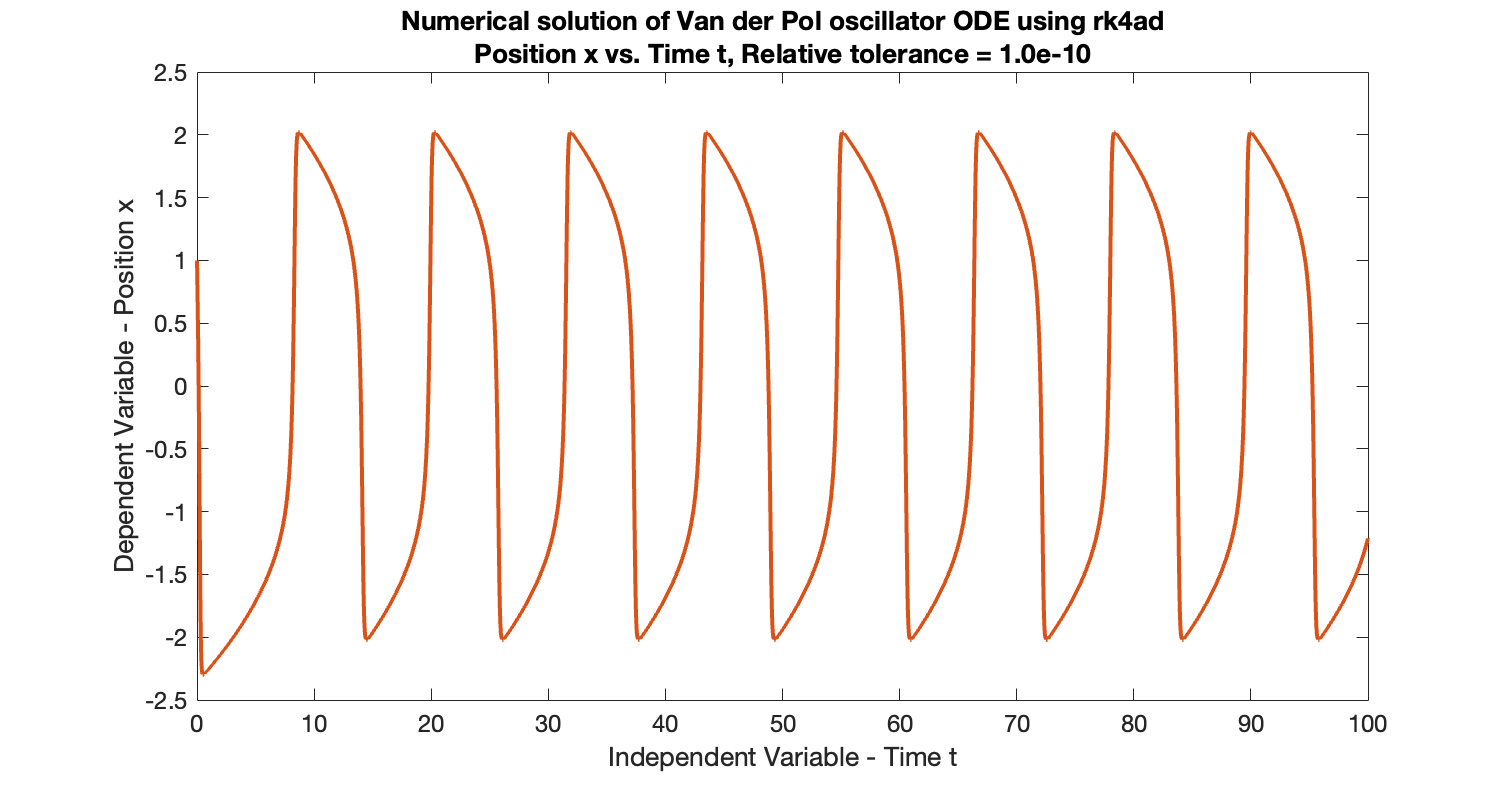
\includegraphics[width=0.9\textwidth]{trk4ad_vdp_1.png}
\caption{Numerical solution of the Van der Pol oscillator ODE computed by \code{rk4ad.m} on the domain
defined by \code{tspan = linspace(0.0, 100, 4097)} with \code{reltol = 1.0e-10}.}
\label{trk4ad_vdp_1_fig}
\end{figure}

\begin{figure}[H]
\centering
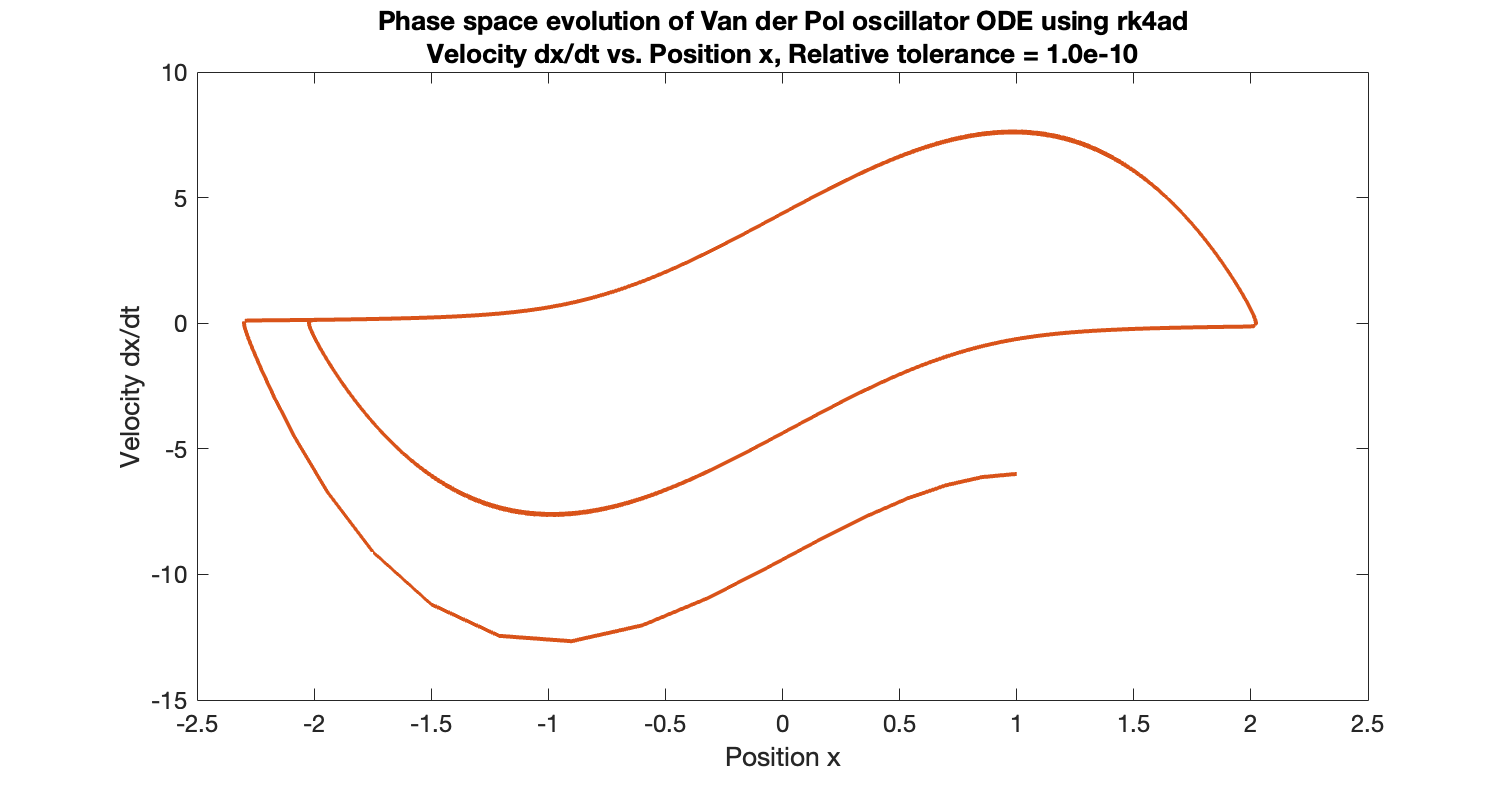
\includegraphics[width=0.9\textwidth]{trk4ad_vdp_2.png}
\caption{Phase space evolution of the Van der Pol oscillator ODE computed by \code{rk4ad.m} on the domain
defined by \code{tspan = linspace(0.0, 100, 4097)} with \code{reltol = 1.0e-10}.}
\label{trk4ad_vdp_2_fig}
\end{figure}

%%%%%%%%%%%%%%%%%%%%%%%%%%%%%%%%%%%%%%%%%%%%%%%%%%%%%%%%%%%%%%%%%%%%%%%%%%%%%%%%%%%%%%%%%%%%%%%%%%%%%%%
% Conclusions
%%%%%%%%%%%%%%%%%%%%%%%%%%%%%%%%%%%%%%%%%%%%%%%%%%%%%%%%%%%%%%%%%%%%%%%%%%%%%%%%%%%%%%%%%%%%%%%%%%%%%%%
\subsection*{Conclusions}

By testing with the scripts described previously, the functions \code{rk4step}, \code{rk4}, and 
\code{rk4ad} were determined to work as expected. \code{rk4step} was shown to be accurate
to $O(\Delta t^5)$, and \code{rk4} was shown to be accurate to $O(\Delta t^4)$. From Figure 
\ref{trk4ad_sho_2_fig}, we can conclude that the approximation \code{rk4ad} produces is accurate to 
\textit{at least} $O(\Delta t^4)$ where $\Delta t$ represents the spacing between adjacent elements in 
\code{tspan}. However, since \code{reltol} can be manually adjusted the accuracy increased further. 

The MATLAB implementation of \code{rk4ad} can likely be made more concise and efficient if time is taken 
to improve it. Additionally, other implementations of \code{rk4ad} could vary the step size differently 
depending on the estimated error. 

Generative AI was used only for assistance in typesetting this document for this homework assignment. 

\pagebreak

%%%%%%%%%%%%%%%%%%%%%%%%%%%%%%%%%%%%%%%%%%%%%%%%%%%%%%%%%%%%%%%%%%%%%%%%%%%%%%%%%%%%%%%%%%%%%%%%%%%%%%%
% Appendices
%%%%%%%%%%%%%%%%%%%%%%%%%%%%%%%%%%%%%%%%%%%%%%%%%%%%%%%%%%%%%%%%%%%%%%%%%%%%%%%%%%%%%%%%%%%%%%%%%%%%%%%

\subsection*{Appendix A - rk4step.m Code}
\lstinputlisting{../src/rk4step.m}
\pagebreak

\subsection*{Appendix B - trk4step.m Code}
\lstinputlisting{../src/trk4step.m}
\pagebreak

\subsection*{Appendix C - rk4.m Code}
\lstinputlisting{../src/rk4.m}
\pagebreak

\subsection*{Appendix D - trk4\_sho.m Code}
\lstinputlisting{../src/trk4_sho.m}
\pagebreak

\subsection*{Appendix E - trk4\_vdp.m Code}
\lstinputlisting{../src/trk4_vdp.m}
\pagebreak

\subsection*{Appendix F - rk4ad.m Code}
\lstinputlisting{../src/rk4ad.m}
\pagebreak

\subsection*{Appendix G - trk4ad\_sho.m Code}
\lstinputlisting{../src/trk4ad\_sho.m}
\pagebreak

\subsection*{Appendix H - trk4ad\_vdp.m Code}
\lstinputlisting{../src/trk4ad\_vdp.m}
\pagebreak

\end{document}